\documentclass[11pt]{standalone}

\usepackage{wasysym}
\usepackage{ifthen}
\usepackage{tikz} 
\usetikzlibrary{shapes.misc}
\usetikzlibrary{arrows,arrows.meta}
\usetikzlibrary{calc,intersections, patterns, math}

\definecolor{pfeil}{RGB}{168,167,167}
\definecolor{petrol}{RGB}{0, 118, 136}
\definecolor{darkgoldenrod}{RGB}{184, 134, 11}
\colorlet{petrol-lighter}{petrol!40}
\colorlet{darkgoldenrod-lighter}{darkgoldenrod!40}

\begin{document}

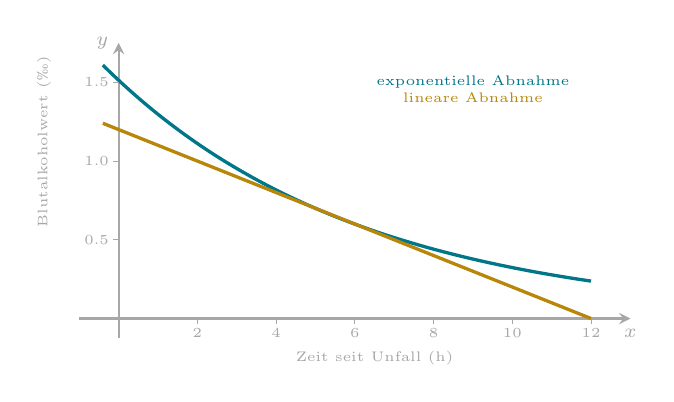
\begin{tikzpicture}[pfeil]

    % \draw[thick, fill=petrol!20, draw=petrol-lighter, rounded corners=2ex, opacity=0.5] (0,0) rectangle ++ (1.5,3.5);
    % \draw[thick, fill=darkgoldenrod!20, draw=darkgoldenrod-lighter, rounded corners=2ex, opacity=0.5] (5,0) rectangle ++ (1.5,3.5);

    \draw[thick, -stealth] (-0.5,0) -- (6.5,0) node[below]{$\scriptstyle x$}; % 1 sind 2 Stunden
	\draw[thick, -stealth] (0,-0.25) -- (0,3.5) node[left]{$\scriptstyle y$};
	
	\draw[very thick,domain=-0.2:6.0, smooth, samples=50, petrol] plot(\x,{2*(1.513*(6/7)^(2*\x))}) ;
	\draw[very thick,domain=-0.2:6.0, smooth, samples=50, darkgoldenrod] plot(\x,{2*(-0.2*\x+1.2)}) ;

    \node[petrol] at (4.5,3) {\tiny exponentielle Abnahme};
    \node[darkgoldenrod] at (4.5,2.8) {\tiny lineare Abnahme};

    \node[rotate=90] at (-0.95,2.25) {\tiny Blutalkoholwert (\permil)};
    \node[] at (3.25,-0.5) {\tiny Zeit seit Unfall (h) };

    \foreach \x in {2,4,...,12}{
        \draw[] (\x/2 ,0) -- ++ (0,-0.075) node[below, yshift=0.75mm] {\tiny \x} ;
    }

    \foreach \x in {0.5,1.0,...,1.5}{
        \draw[] (0, \x*2) -- ++ (-0.075,0) node[left, xshift=0.75mm] {\tiny \x} ;
    }


\end{tikzpicture}

\end{document}
